\chapter{Sprint 1}

\section*{Introduction}
In this Sprint we go through the planning, analyzing, and implementing phases of the configuration module.
\subsubsection*{Purpose of the configuration module}
This module is dedicated to the platform administrator. \\
It is a parameter setting module that facilitates the internal configuration of the application, mainly by managing :\\
\begin{itemize}
    \item The different travel policies
    \item The destinations and their requirements (visa and vaccines)
    \item The administrative grades
\end{itemize}\\
\subsubsection*{Actors}
There is a single actor that can access and interact with this module:
\begin{itemize}
    \item Admin: The platform's administrator
\end{itemize}\\
\section{Sprint backlog}
The following table summarizes the tasks that we are responsible for carrying out 
\begin{center}
\begin{longtable}{|p{1cm}|p{6,25cm}|p{0,7cm}|p{6,25cm}|p{0,8cm}|}
\caption{ Project backlog }
\hline
\textbf{US ID} 
&\textbf{User Story}
&\textbf{T ID}
&\textbf{Task}
&\textbf{Esti- ma- tion}
\\
\hline
\multirow{ 3}{*}{0}
&\multirow{3}{*}{Storyless}
&0.1
&Class diagram
&8h\\\cline{3-5}
&
&0.2
&Use case diagram
&8h\\\cline{3-5}
&
&0.3
&Documenting progress
&2h\\\cline{3-5}
\hline
1
&As an Administrator , Agent , Manager or User, I want to be able to log-in
&1
&Setup Odoo
&8h
\\\hline


\multirow{ 6}{*}{8}
&\multirow{6}{=}{As an Administrator , I want to be able to view, create, edit, delete and import new countries}
&8.1
&Create the «country» model
&8h\\\cline{3-5}
&
&8.2
&Create the view
&2h\\\cline{3-5}
&
&8.3
&Create security rules
&1h\\\cline{3-5}
&
&8.4
&Create the «Destinations» menu item
&30m\\\cline{3-5}
&
&8.5
&Create the «Airport» model
&30m\\\cline{3-5}
&
&8.6
&Create the «State» model
&30m\\\cline{3-5}
\hline


\multirow{ 5}{*}{9}
&\multirow{5}{=}{As an Administrator , I want to be able to view, create, edit, delete and import flight policies}
&9.1
&Create the «flight\_policy» model
&8h\\\cline{3-5}
&
&9.2
&Create the view
&2h\\\cline{3-5}
&
&9.3
&Create security rules
&1h\\\cline{3-5}
&
&9.4
&Create the «Policies» menu item
&30m\\\cline{3-5}
&
&9.5
&Create «flight\_class\_rules» model
&4h\\\cline{3-5}
\hline


\multirow{ 3}{*}{10}
&\multirow{3}{=}{As an Administrator , I want to be able to view, create, edit, delete and import hotel reservation policy}
&10.1
&Create the «hotel\_policy» model
&8h\\\cline{3-5}
&
&10.2
&Create the view
&2h\\\cline{3-5}
&
&10.3
&Create security rules
&1h\\\cline{3-5}

\hline
\multirow{3}{*}{11}
&\multirow{3}{=}{As an Administrator , I want to be able to view, create, edit, delete and import per diem policy}
&11.1
&Create the «perdiem\_policy» model
&8h\\\cline{3-5}
&
&11.2
&Create the view
&2h\\\cline{3-5}
&
&11.3
&Create security rules
&1h\\\cline{3-5}
\hline

\multirow{ 4}{*}{12}
&\multirow{4}{=}{As an Administrator , I want to be able to view, create, edit, delete and import visa model}
&12.1
&Create the «visa» model
&8h\\\cline{3-5}
&
&12.2
&Create the view
&2h\\\cline{3-5}
&
&12.3
&Create security rules
&1h\\\cline{3-5}
&
&12.4
&Create model relations
&2h\\\cline{3-5}
\hline


\multirow{ 4}{*}{13}
&\multirow{4}{=}{As an Administrator , I want to be able to view, create, edit, delete and import vaccins}
&13.1
&Create the «vaccine» model
&4h\\\cline{3-5}
&
&13.2
&Create the view
&1h\\\cline{3-5}
&
&13.3
&Create security rules
&1h\\\cline{3-5}
&
&13.4
&Create the «Vaccine» menu item
&30m\\\cline{3-5}

\hline

14
&As an Administrator , I want to be able to attribute vaccines to countries
&14.1
&Create model relation
&2h\\
\hline

15
&As an Administrator , I want to be able to attribute visas to countries
&15.1
&Create model relation
&2h\\
\hline
\\\\

\multirow{5}{*}{16}
&\multirow{5}{=}{As  an  Administrator  ,  I  want  to be able to create , edit and delete administrative grades}
&16.1
&Create the «grade» model
&8h\\\cline{3-5}
&
&16.2
&Create the view
&30m\\\cline{3-5}
&
&16.3
&Create security rules
&1h\\\cline{3-5}
&
&16.4
&Create model relations
&1h\\\cline{3-5}
&
&16.5
&Create the «Grade» menu item
&30m\\\cline{3-5}
\hline

\multirow{ 3}{*}{17}
&\multirow{3}{=}{As an Administrator , I want to be to attribute administrative grades to users}
&17.1
&Add «Grade» field to «hr\_employee» model
&4h\\\cline{3-5}
&
&17.2
&edit «hr\_employee» security rules
&2h\\\cline{3-5}
&
&17.3
&edit «hr\_employee» view
&1h\\\cline{3-5}
\hline

\multirow{ 3}{*}{18}
&\multirow{3}{=}{As an Administrator , I want to be able to create , edit and delete mission types}
&18.1
&Create the «mission\_type» model
&8h\\\cline{3-5}
&
&18.2
&Create the view
&2h\\\cline{3-5}
&
&18.3
&Create security rules
&1h\\\cline{3-5}
\hline
\end{longtable}
\end{center}
\section{Software Design}
The conceptual study conducted at the beginning of an iteration allows us to evaluate the sprint in its early stages by providing a stable reference of conceptual data model and processing to identify potential scenarios. 
    \subsection{Class diagram}
    The following diagram represents the entities manipulated by users as
analysis class diagram
    \begin{figure}[H]
    \begin{center}
        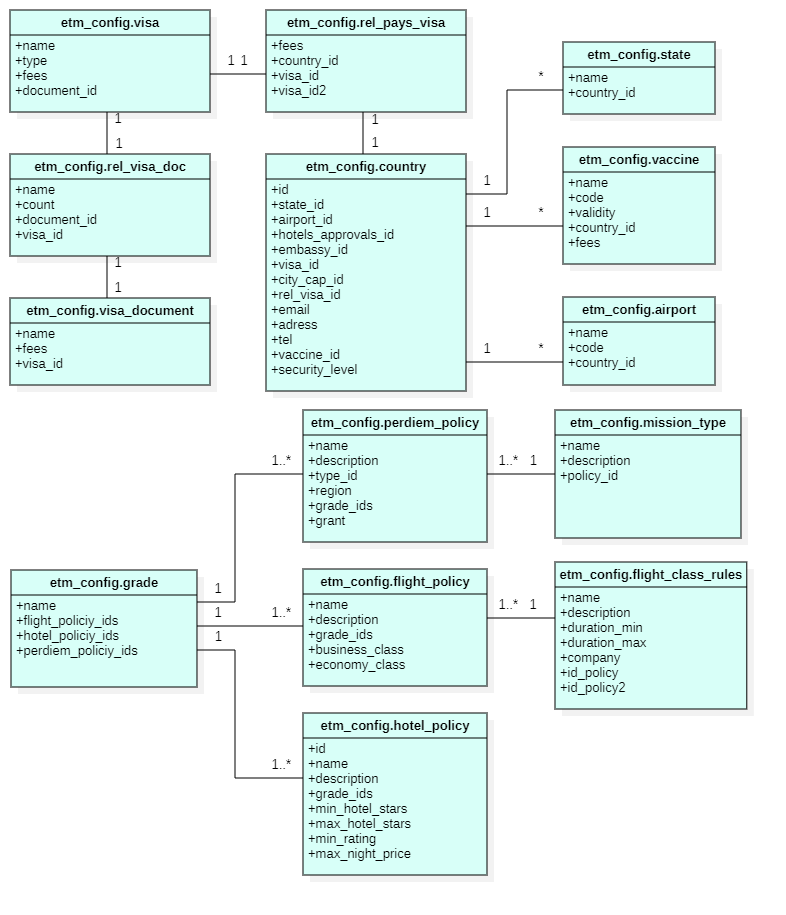
\includegraphics[scale=0.5]{img/sprint1_class.png}
        \caption{Sprint 1 class diagram}
    \end{center}
     \label{fig:my_label}
\end{figure}
    \subsection{Use case diagram}
    The use case diagram below helps to highlight the relationships
functional between the actors and the system under study 
    \begin{figure}[H]
    \begin{center}
        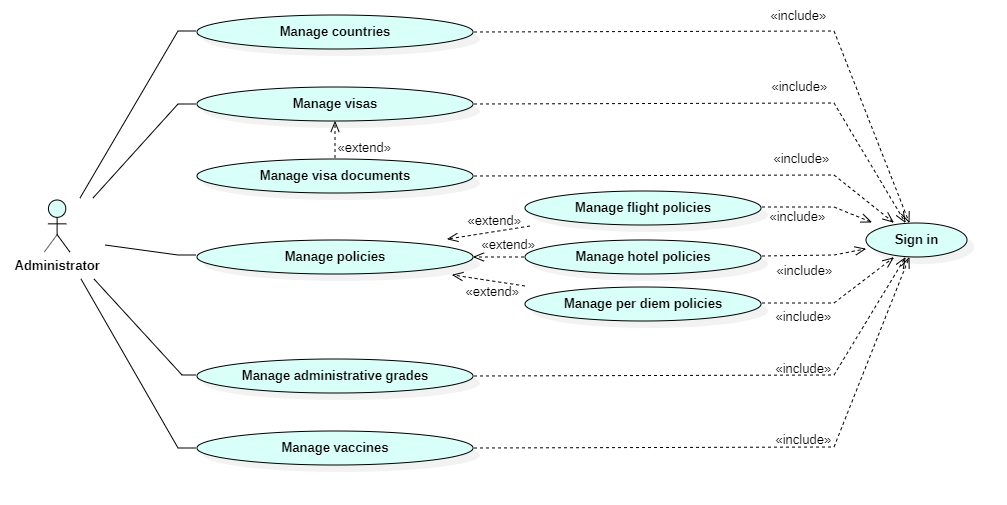
\includegraphics[scale=0.50]{img/UseCaseDiagramSprint1.png}
        \caption{Sprint 1 use case diagram}
    \end{center}
        \label{fig:my_label}
\end{figure}
  \\ In what follows, we will proceed to go in detail on some use cases  


\subsection*{Use case «Manage countries»}
\begin{figure}[H]
    \begin{center}
        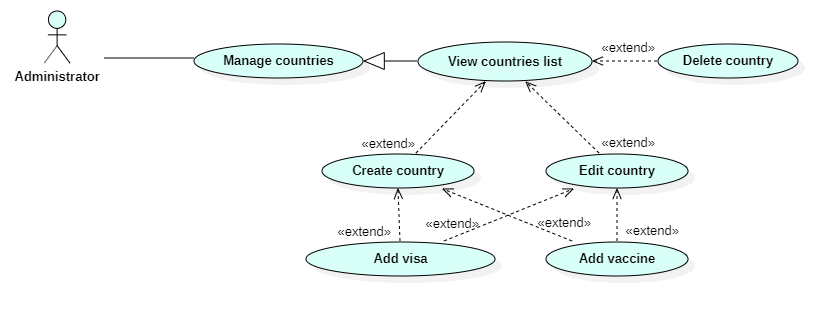
\includegraphics[scale=0.5]{img/sprint1_country_usecase.png}
        \caption{«Manage countries» detailed use case diagram}
    \end{center}
        \label{fig:my_label}
\end{figure} 
    The following table addresses the use case previously illustrated by providing a textual description, post and preconditions as well as the main scenario and the nominal scenario
    \begin{center}
    
\begin{longtable}{|p{4,25cm}|p{9,25cm}|}
\caption{«Manage countries» detailed textual description}
\hline
\textbf{Use Case}&Create country
\\\hline
\textbf{Actors}&Administrator
\hline
\textbf{Pre-condition}&Administrator signed in and viewing countries list
\hline
\textbf{Post-condition}&New country created
\hline
\textbf{Basic path}&
        \begin{itemize}
         \item[1.] The administrator clicks on the button "New"
         \item[2.] The system displays a form to fill out
         \item[3.] The administrator fills the form
         \item[4.] The administrator clicks on the button "Save"
         \item[5.] The system processes the input
         \item[6.] The system saves the new country
         \item[7.] The administrator is sent back to the countries list
     \end{itemize}\\
\hline
\textbf{Alternative path}&
\begin{itemize}
\item 4.Duplicate or missing Data (The administrator is sent back to step 2)

\end{itemize}\\
\hline
\end{longtable}
\end{center}




\subsection*{Use case «Manage visas»}
\begin{figure}[H]
    \begin{center}
        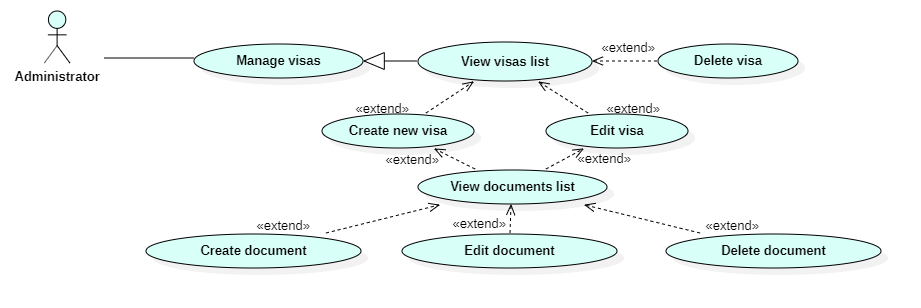
\includegraphics[scale=0.45]{img/sprint1_visa_usecase.png}
        \caption{«Manage visas» detailed use case diagram}
    \end{center}    
\end{figure}
    In the following we will present the sequence diagram to illustrate the relationships between the actor and the different components of our use case from a temporal point of view, focusing on the chronology of the exchanges of messages.
    \begin{figure}[H]
     \begin{center}
        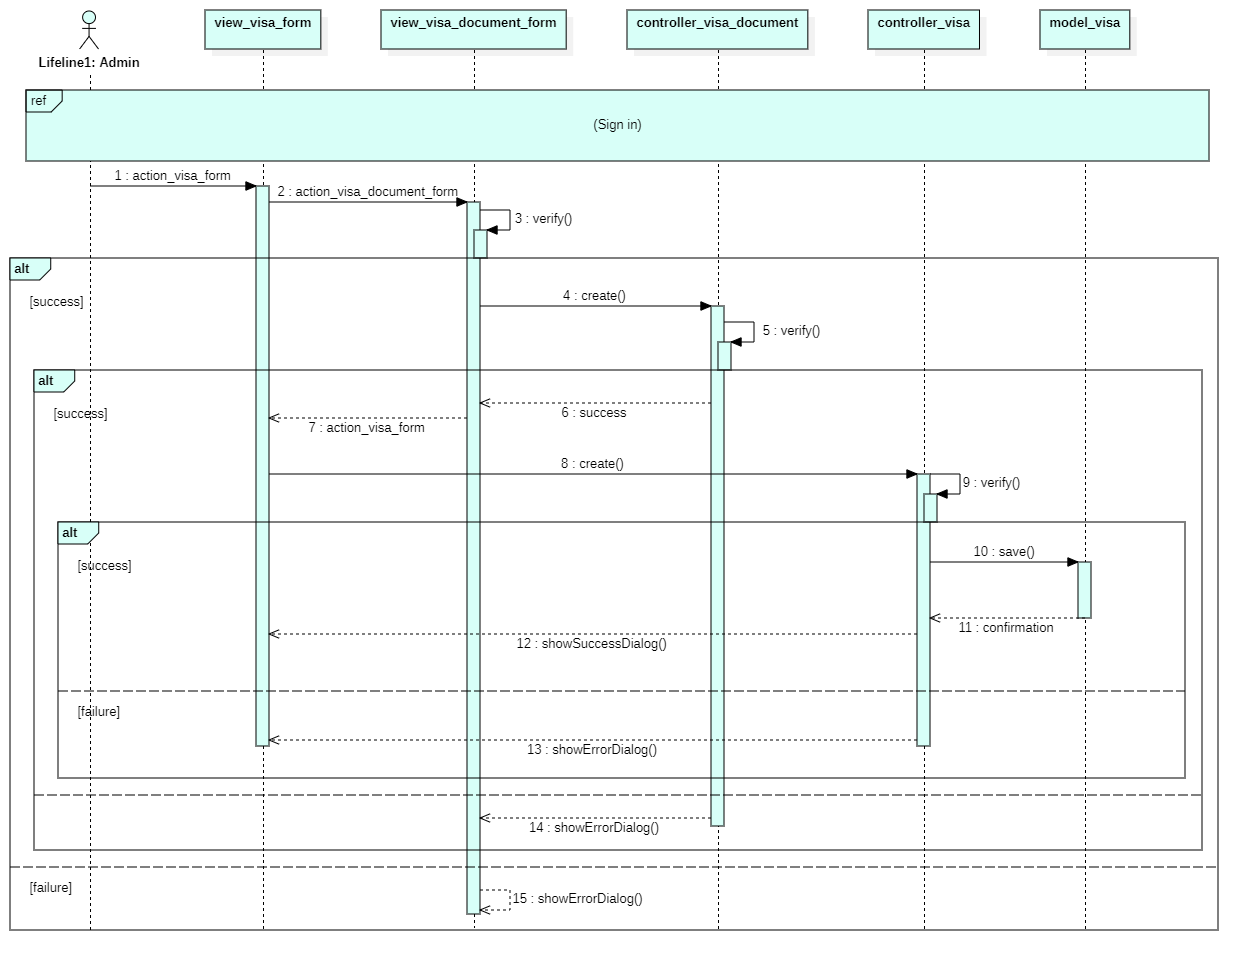
\includegraphics[scale=0.355]{img/sprint1_visa_sequ.png}
        \caption{«Manage visas» sequence diagram}
    \end{center}   
    \end{figure}
    
    
    
    
    
\subsection*{Use case «Manage vaccines»}
\begin{figure}[H]
    \begin{center}
        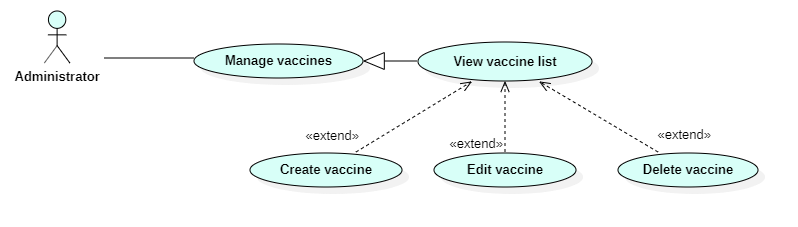
\includegraphics[scale=0.50]{img/sprint1_vaccine_usecase.png}
 \caption{«Manage vaccines» detailed use case diagram}
    \end{center}   
    \end{figure}
      The following table addresses the use case previously illustrated by providing a textual description, post and preconditions as well as the main scenario and the nominal scenario
    \begin{center}
    
\begin{longtable}{|p{4,25cm}|p{9,25cm}|}
\caption{«Manage vaccines» detailed textual description}
\hline
\textbf{Use Case}&Create vaccine
\\\hline
\textbf{Actors}&Administrator
\hline
\textbf{Pre-condition}&Administrator signed in and viewing vaccines list
\hline
\textbf{Post-condition}&New vaccine created
\hline
\textbf{Basic path}&
        \begin{enumerate}
         \item The administrator clicks on the button "New"
         \item The system displays a form to fill out
         \item The administrator fills the form
         \item The administrator clicks on the button "Save"
         \item The system processes the input
         \item The system saves the new vaccine
         \item The administrator is sent back to the countries list
     \end{enumerate}\\
\hline
\textbf{Alternative path}&
\begin{itemize}
\item 4.Duplicate or missing Data (The administrator is sent back to step 2)

\end{itemize}\\
\hline
\end{longtable}
\end{center}  
    
    
    
    
    
    
    
\subsection*{Use case «Manage policies»}
\begin{figure}[H]
    \begin{center}
        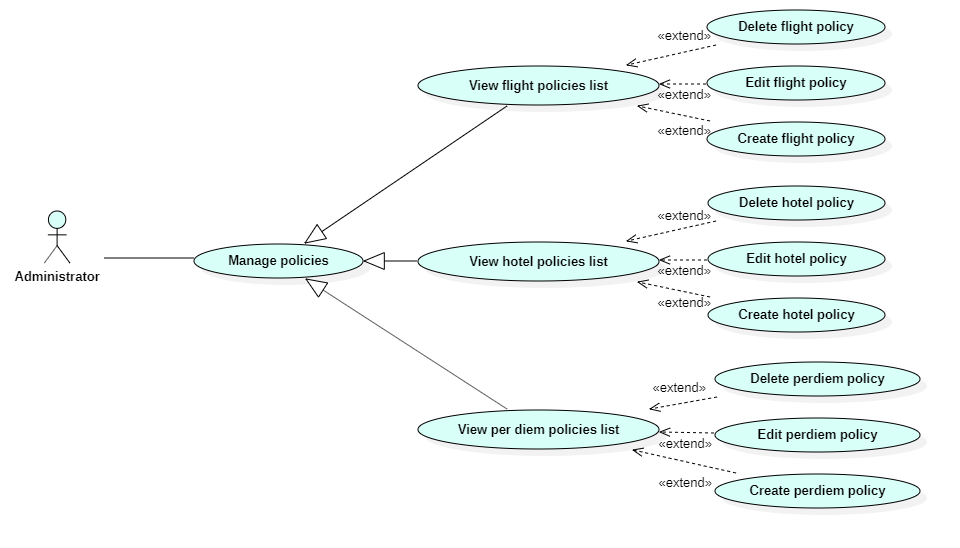
\includegraphics[scale=0.50]{img/sprint1_policy_usecase.png}
         \caption{«Manage policies» detailed use case diagram}
    \end{center}   
    \end{figure}
    
    
        \begin{center}
    
\begin{longtable}{|p{3.2cm}|p{10cm}|}
\caption{«Manage policies» detailed textual description}
\hline
\textbf{Use Case}&Edit flight policy
\\\hline
\textbf{Actors}&Administrator
\hline
\textbf{Pre-condition}&Administrator signed in and flight policies list
\hline
\textbf{Post-condition}&Flight policy edited\\
\hline
\textbf{Basic path}&
        \begin{enumerate}
         \item The administrator clicks on the button "New"
         \item The system displays a form to fill out
         \item The administrator fills the form
         \item The administrator selects at least one of each policy
         \item The administrator clicks on the button "Save"
         \item The system processes the input
         \item The system saves the new vaccine
         \item The administrator is sent back to the countries list
     \end{enumerate}\\
\hline
\textbf{Alternative path}&
\begin{itemize}
\item 6.Duplicate or missing Data (The administrator is sent back to step 3)
\item 4.No policy exist and the user is prompted to go to the policy creation form
\end{itemize}\\
\hline
\end{longtable}
\end{center}  




\subsection*{Use case «Manage administrative grades»}
\begin{figure}[H]
    \begin{center}
        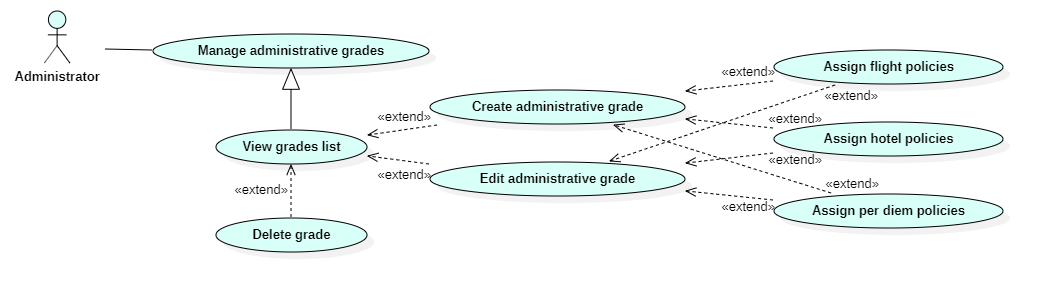
\includegraphics[scale=0.50]{img/sprint1_grade_usecase.png}
        \caption{«Manage administrative grades» detailed use case diagram}
    \end{center}   
    \end{figure}
    
    The following table addresses the use case previously illustrated by providing a textual description,post and preconditions as well as the main scenario and the nominal scenario
    
            \begin{center}
    
\begin{longtable}{|p{3.2cm}|p{10cm}|}
\caption{«Manage administrative grades» detailed textual description}
\hline
\textbf{Use Case}&Create administrative grade
\\\hline
\textbf{Actors}&Administrator
\hline
\textbf{Pre-condition}&Administrator signed in and viewing grades list
\hline
\textbf{Post-condition}&New grade created
\hline
\textbf{Basic path}&
        \begin{enumerate}
         \item The administrator selects a policy
         \item The system displays the policy information
         \item The administrator clicks on the button "Edit"
         \item The system displays a filled form
         \item The administrator edits the fields
         \item The administrator clicks on the button "Save"
         \item The system processes the input
         \item The system saves the new policy
         \item The administrator is sent back to the flight policies list
     \end{enumerate}\\
\hline
\textbf{Alternative path}&
\begin{itemize}
\item 7.Duplicate or missing Data (The administrator is sent back to step 3)
\item 6.form not edited (System skips to step 9)
\end{itemize}\\
\hline
\end{longtable}
\end{center}  



\section{Implementation}
This section presents some user interfaces of the module with screenshots to further clarify our work. The figures below present these interfaces, starting with the first figure which shows the authentication interface.

\begin{figure}[H]
    \centering
    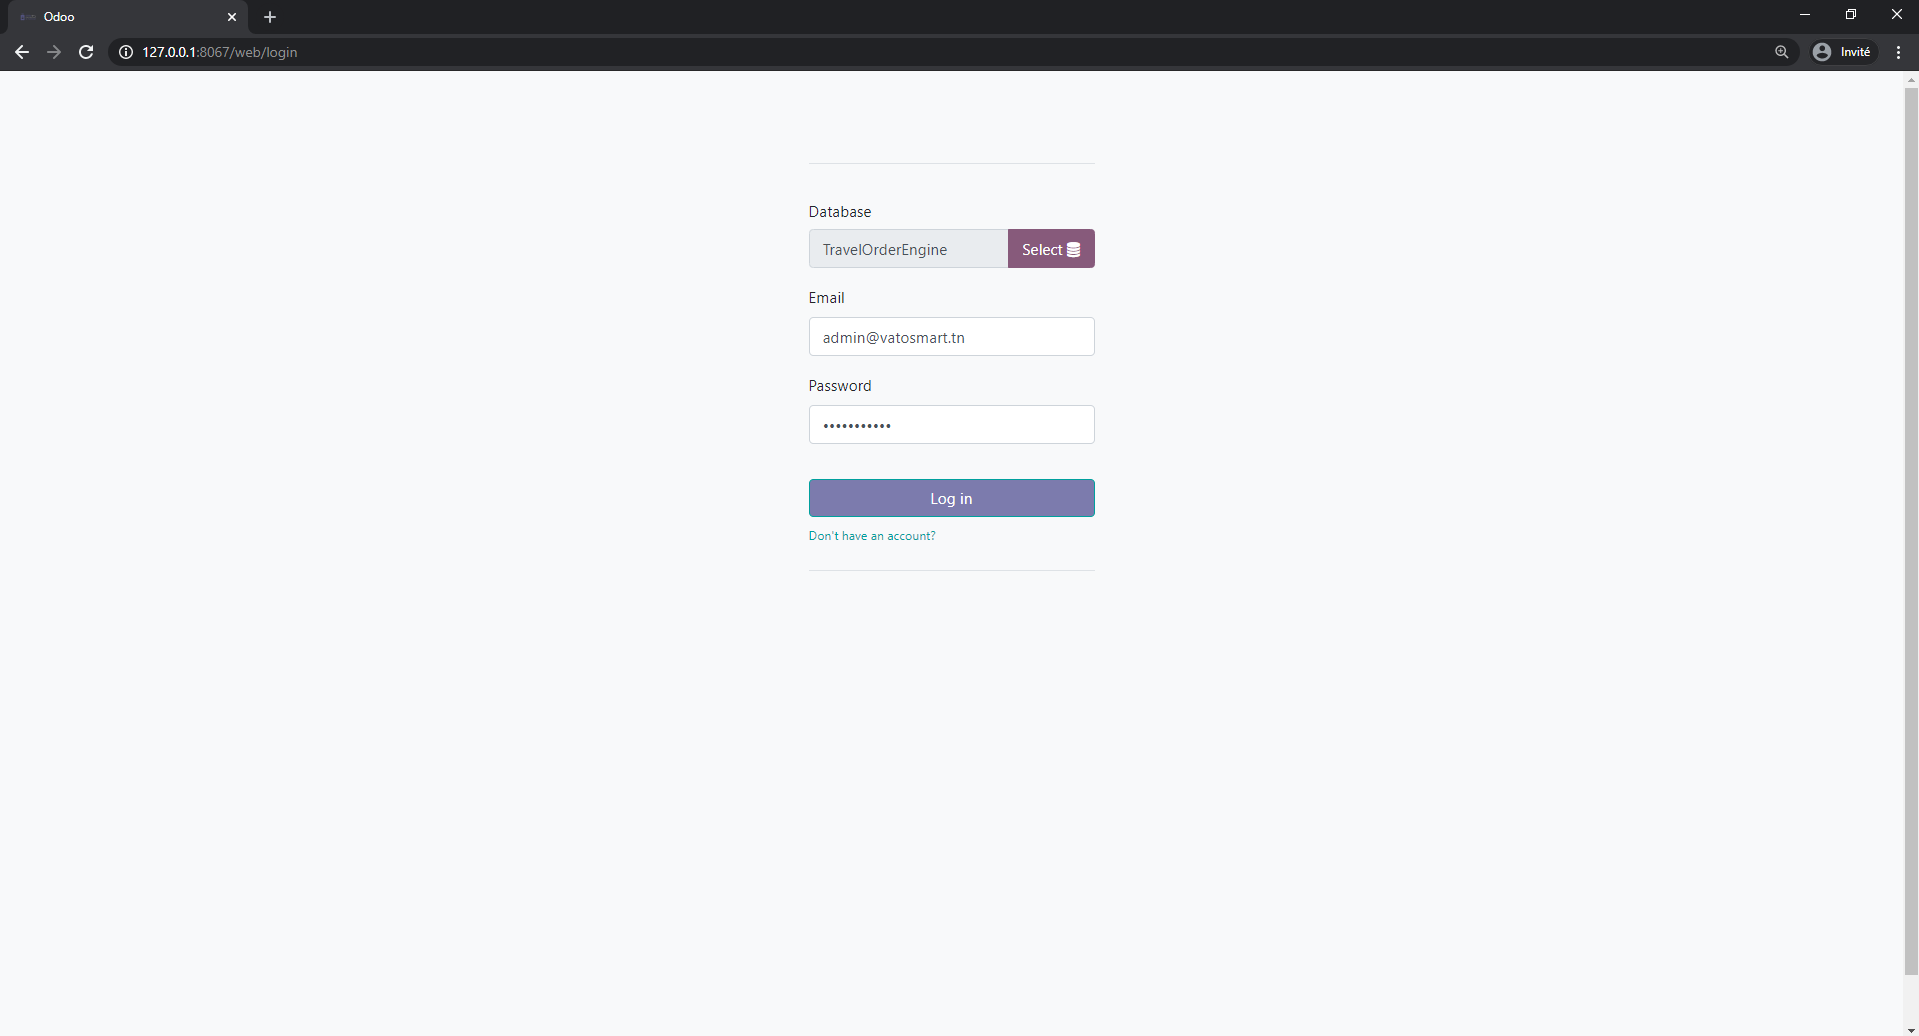
\includegraphics[scale=0.30]{img/c_auth.png}
    \caption{Interface <<Authentication>>}
    \label{fig:my_label}
\end{figure}

And on the next figure, we will show the main menu of this module, this navigation bar remains accessible from all views on this module.
\begin{figure}[H]
    \centering
    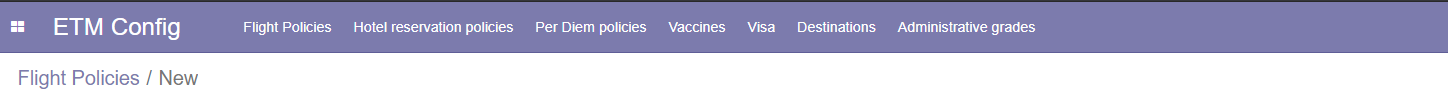
\includegraphics[scale=0.43]{img/c_config_menu.png}
    \caption{Configuration module menu}
    \label{fig:my_label}
\end{figure}
In this figure we will show the Countries list view, all countries are listed on this tree view and we can find our operations on the buttons above them. The administrator is the only actor able to access these views
\begin{figure}[H]
    \centering
    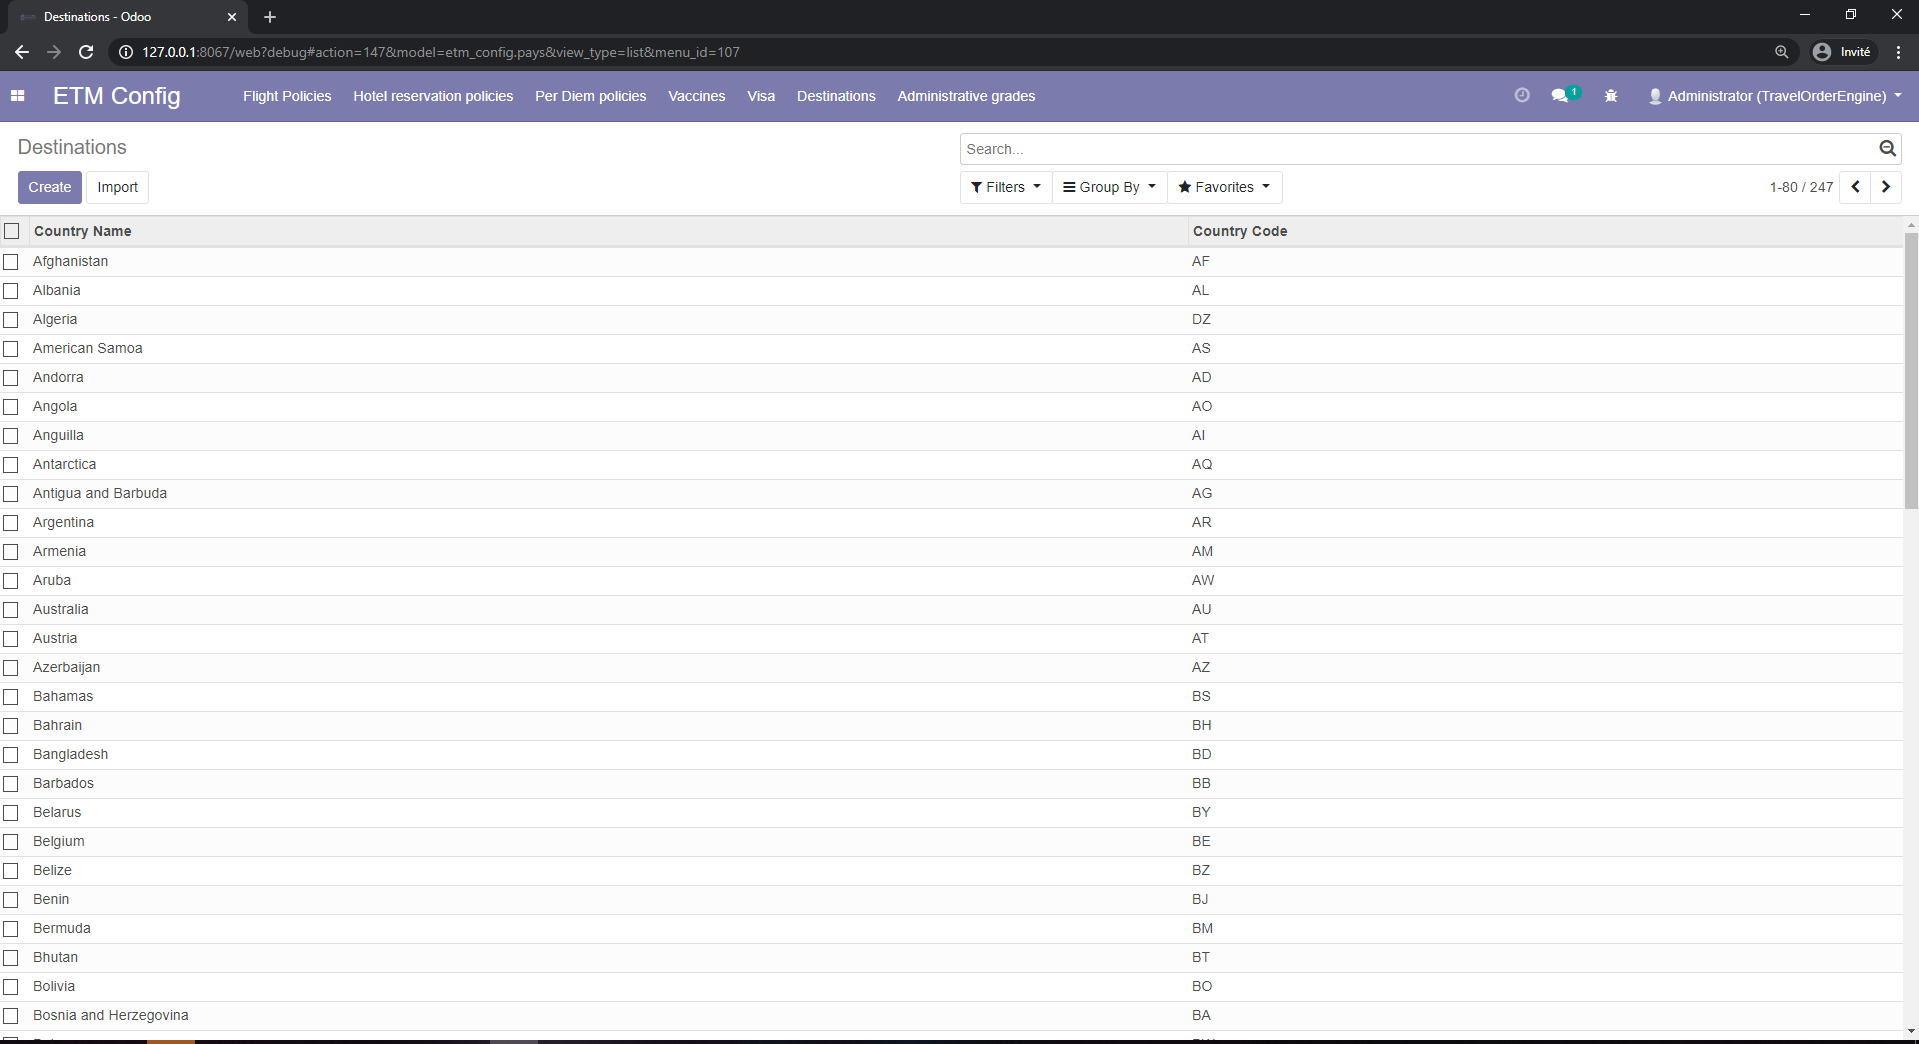
\includegraphics[scale=0.32]{img/c_country_list.png}
    \caption{Countries list view}
    \label{fig:my_label}
\end{figure}
In this figure we will go over the flight policy view, here we can Edit or Duplicate the policy we are viewing or we can create a new one
\begin{figure}[H]
    \centering
    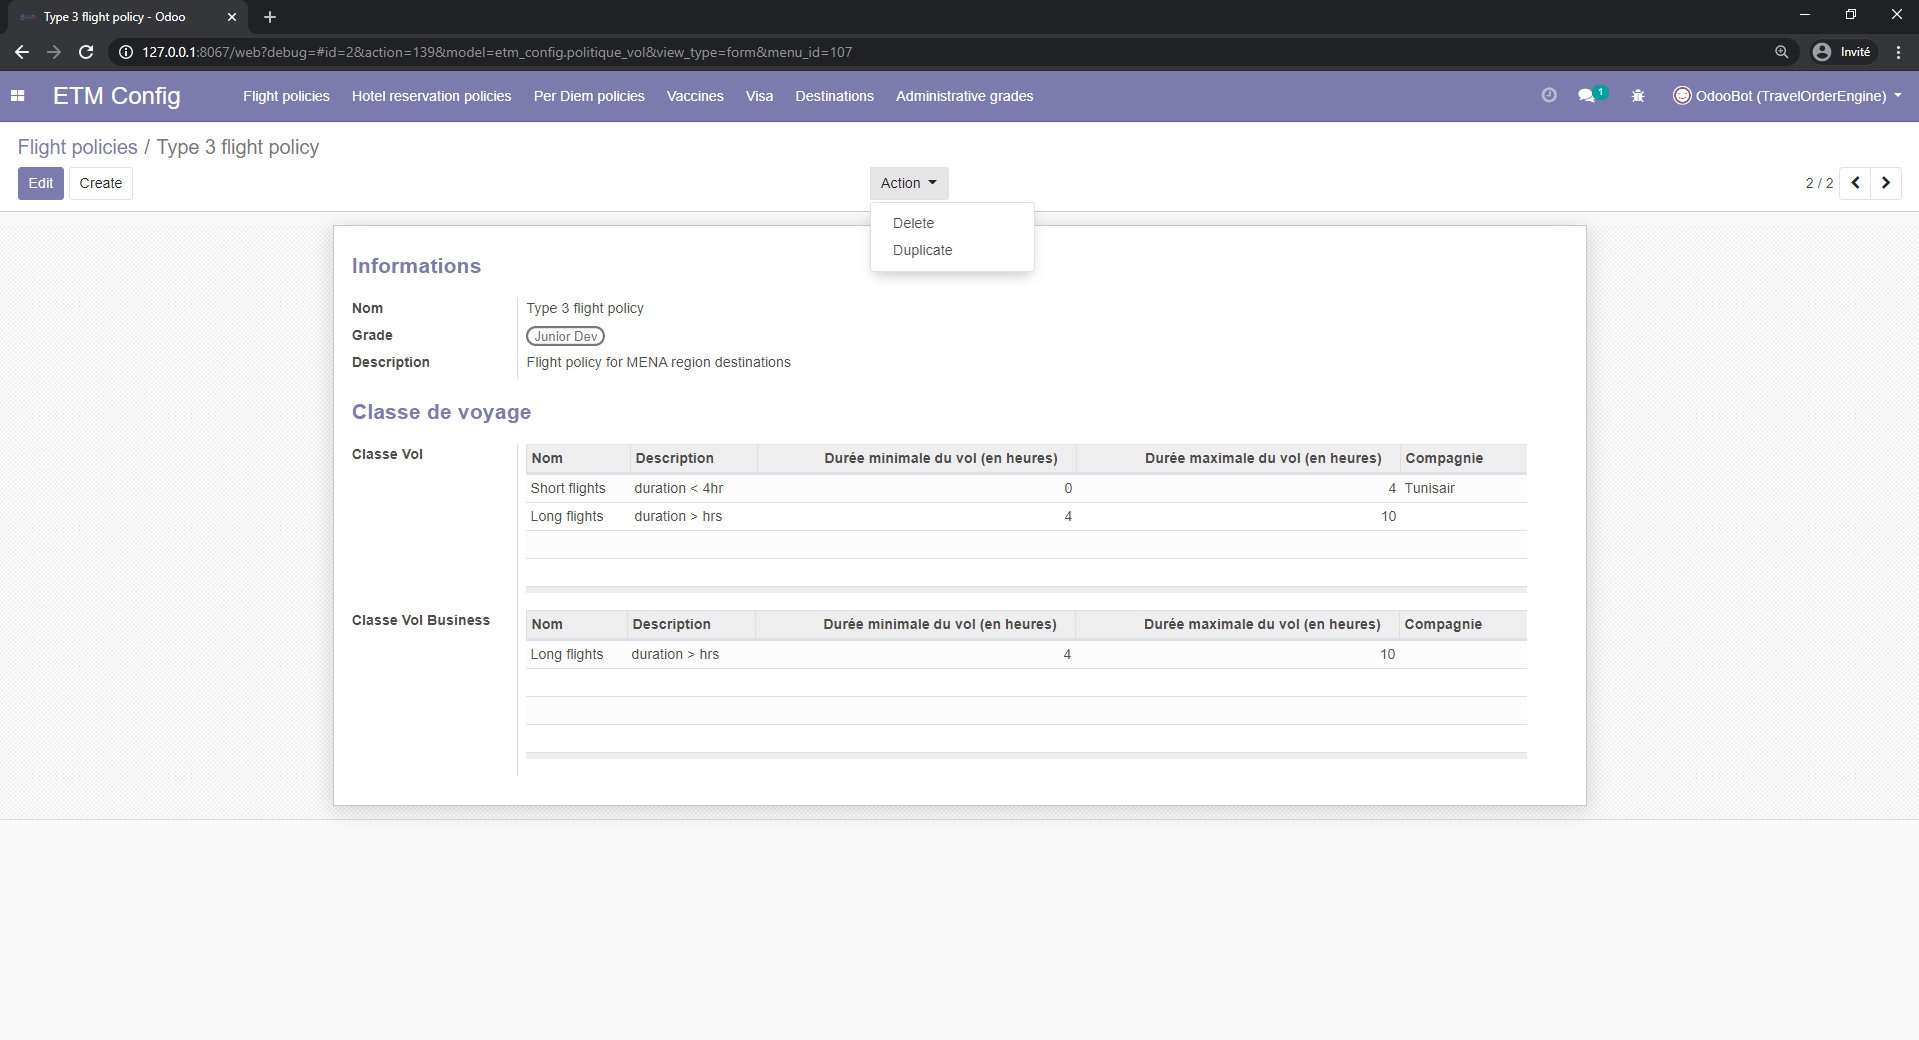
\includegraphics[scale=0.32]{img/c_flight_policy.png}
    \caption{Countries list view}
    \label{fig:my_label}
\end{figure}
\section*{Conclusion}
In this chapter we have discussed the sprint1 of our project which concerns the design, development and implementation of a first module our project which is the configuration module . This sprint was spread over one month. At the beginning of this sprint we set objectives to be reached. We started with the elaboration of the Backlog sprint afterwards we started a design phase before starting the development. \\During the development phase there was a daily meeting of the project working committee where everyone presented what they had done the day before, what they intended to do and if they faced any obstacles.\\ We closed this chapter with a section called realization where we presented some interfaces of the first increment of our project.\\
In what follows we will begin the second phase of the project, namely the design, development and implementation of a second module which concerns the management of Employees.
